\documentclass{article}
\usepackage{geometry}
\usepackage{natbib}
\usepackage{amssymb}
\usepackage{amsmath}
\usepackage{graphicx}
\usepackage{subfig}
\usepackage{hyperref}
\usepackage{textcomp}
\usepackage{array}
\usepackage{booktabs}
\usepackage{makecell}
\usepackage[singlelinecheck=false]{caption}
\usepackage{comment}

\geometry{
	a4paper,
	total={170mm,257mm},
	left=30mm,
	top=30mm,
	bottom=20mm,
	right=20mm
}
\title{
	Relatório - Modelagem Matemática\\
	Estudo de População de Aves na Amazônia \\
	\large Usando o Modelo de Reação-Difusçao para avaliar sobrevida de populações em manchas de floresta em áreas desmatadas.
}
\date{2024-07-20}
\author{Paulo Roberto Rodrigues da Silva Filho\\Pedro Paulo Dantas Silva Martins\\Vicente Alves da Silva Sirufo}

\newcommand\R{\mathbb{R}}

\begin{document}
	\renewcommand{\figurename}{Figura}
	\renewcommand{\tablename}{Tabela}
	\renewcommand{\cellalign}{tl}
	\renewcommand{\theadalign}{tl}
	
	\graphicspath{ {./imagens/} }
	\maketitle
	\tableofcontents
	
	\section{Introdução}
	
	\paragraph{}
	Em função do processo de desmatamento da Amazônia, percebeu-se que, dentro das regiões desmatadas, formam-se manchas florestadas isoladas. Tais manchas podem ou não ser adequadas para a sustentação de populações animais. O modelo utilizado para se avaliar a capacidade de tais manchas sustentarem populações é o Modelo de Reação/Difusão, regido pela Equação Diferencial Parcial (EDP) FKPP (Modelo Fischer-Kolmogorov-Petrovsky-Piskunov). Foi avaliada a capacidade de sustentação de população de uma única espécie e, também, de duas espécies em competição.
	
	\paragraph{}
	Para entender o problema, vamos, primeiro, apresentar um diagrama, representando a floresta e áreas desmatadas, conforme pode ser visto na Figura \ref{fig:efloresta}. Conforme essa figura, temos uma grande área de floresta e uma área desmatada que possui manchas de floresta. A área desmatada pode suportar uma população mínima dos animais em estudo, ou suportar uma população temporária de forma que permita a migração dessas populações entre a área de floresta virgem e as manchas na área desmatada.
	
	\paragraph{}
	Uma vez dada essa representação de ambiente, padrão, podemos utilizar o Modelo de Reação-Difusão, assumindo que, entrando uma determinada população em uma mancha de floresta - ou estando essa população lá isolada, antes do processo de desmatamento - há condições de a população se reproduzir dentro dessa área, estando sujeita a restrições do meio, cooperação e competição intra-específica.
	
	\paragraph{}
	Já no caso de duas populações concorrendo na mesma região, devemos também assumir que a região desmatada tenha capacidade de suportar uma quantidade muito baixa dessas populações, de forma que a hipótese da difusão faça sentido. Fazemos, então, uma análise de ambas as populações em conjunto, em competição.
	
	\paragraph{}
	Tanto no caso da população isolada, quanto na de duas populações, a geometria das manchas (tamanho) e características intrínsecas delas permitem definir uma capacidade de carregamento das populações, que afetam as dinâmicas populacionais. A identificação de um tamanho mínimo de mancha e o isolamento dessa mancha em relação à área florestada, ou a outras manchas também são características a relevantes para o estudo do problema.
	
	\begin{figure}[h]
		\centering
		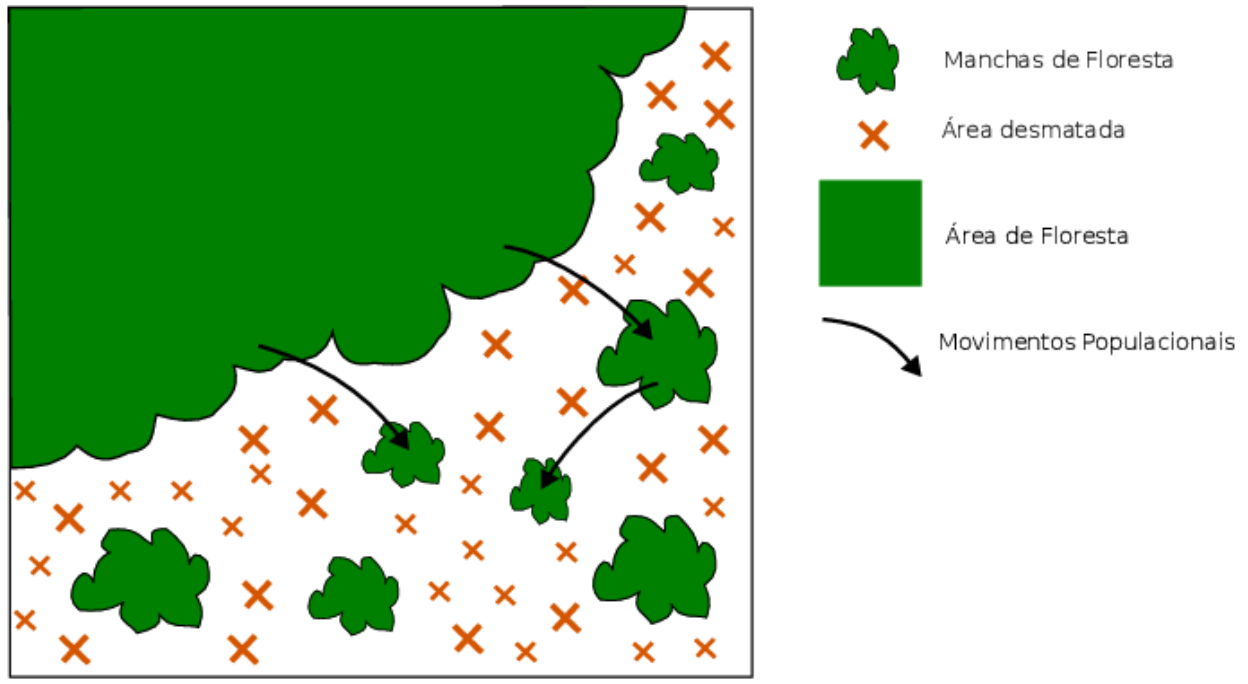
\includegraphics[scale=0.3]{Esquema-Floresta}
		\caption{Representação de área florestada e de manchas de floresta. A área florestada pode ser imaginada como uma mancha de floresta de tamanho infinito, ou, apenas, uma área de tamanho grande o suficiente para ser considerada infinita.}
		\label{fig:efloresta}
	\end{figure}
	
	\section{Modelagem}
	
	\paragraph{}
	Agora vamos apresentar os dois modelos avaliados, o modelo de uma população e o modelo de duas populações. Para ambos os casos são usados variantes da EDP FKPP, apresentadas tais variantes caso a caso.
	
	\subsection{Caso 1: Uma única população}
	
	\paragraph{}
	Para o caso de uma população, o modelo considerado foi FKPP com um termo difusivo (termo de segunda ordem) e os termos reativos, com cooperação (termo linear) e com competição (termo quadrático), sobre uma população $u$:
	
	$$ \frac{\partial u(x,t)}{\partial t} = \alpha u - \beta u^2 + D \frac{\partial^2 u}{\partial x^2}  $$
	
	\paragraph{}
	Com as condições de contorno de Dirichlet:
	
	$$u(x=0,l) = 0 $$
	
	\paragraph{}
	Sendo:
	
	\begin{itemize}
		\item \textbf{u(x,t)}: a população presente na posição espacial e no tempo, na mancha de floresta ou em uma área florestada.
		\item \textbf{D}: taxa de difusividade da população - unidade: \textbf{comprimento\textsuperscript{2}/tempo}.
		\item \textbf{a}: Taxa de cresimento populacional da espécie - unidade: \textbf{1/tempo}
		\item \textbf{b}: Se \textbf{1/C} é a capacidade de carregamento de uma população para uma mancha ou região de floresta, então $C=\frac{b}{a}$, de forma que \textbf{b} indica as condições que atrapalhem o crescimento populacional, como geometria da região de mancha, competição por comida, entre outras.
		\item \textbf{l}: Comprimento (não adimensionalizado) da mancha ou região florestada
	\end{itemize}
	
	\paragraph{}
	Para facilitar a análise, as seguintes transformações são feitas, para se adimensionalizar a equação e, então, avaliar as suas propriedades:
	
	$$ x = x' \sqrt{\frac{D}{a}} $$
	$$ \partial_x = \partial_{x'} \sqrt{\frac{a}{D}} $$
	$$l = L \sqrt{\frac{D}{a}}$$
	$$t = t' \frac{1}{a}$$
	$$\partial_t = \partial_{t'}a$$
	
	\paragraph{}
	Depois, retornando o nome da variável de distância de \textbf{x'} para \textbf{x} e de tempo de \textbf{t'} para \textbf{t}, temos a nova equação:
	
	$$ \frac{\partial u(x,t)}{\partial t} =  \frac{\partial^2 u}{\partial x^2} + u(x,t) - C u^2(x,t)   $$
	
	$$ C(x) =  \begin{cases}
		C_1, & \text{se } |x| < L/2 \\
		C_0, & \text{se } |x| > L/2
	\end{cases}$$
	
	\paragraph{}
	Onde $C_1$ e $C_0$ são a capacidade de carregamento da região interna e externa, respectivamente, de forma que espera-se que a região interna assuma um regime estacionário enquanto a população externa vá assintoticamente para $1/C_0$
	
	\paragraph{}
	Fazemos a seguinte transformação para auxiliar na resolução da EDP:
	
	$$ u = \frac{3}{2} \frac{\phi}{C_1}, $$
	
	$$ \frac{\partial \phi}{\partial t} = \frac{\partial^2\phi }{\partial x^2} + \phi - \frac{3}{2} k*(x)\phi^2 $$
	
	$$ k(x) =  \begin{cases}
		k = \frac{C_0}{C_1}, & \text{se } |x| > L/2 \\
		1, & \text{se } |x| < L/2
	\end{cases}$$
	
	\paragraph{}
	É importante ressaltar que \textbf{k} pode ser interpretado como um indicador do nível de "isolamento" da região interna, como o quão difícil é sair da região ideal ou o quanto a região interna é mais atrativa do que a externa.
	
	\paragraph{}
	Como $\phi$ é uma função contínua e simétrica, e $\frac{2}{3}k$ é uma solução para a parte externa, temos as seguintes condições:
	
	$$\phi_{xx} + \phi - \frac{3}{2}k\phi^2 = 0, \quad x < L/2,$$
	$$\phi_{xx} + \phi - \frac{3}{2}k\phi^2 = 0, \quad 0 > x > -L/2,$$
	$$\phi^o\left(-\frac{L}{2}, \cdot \right) = \phi^i\left(-\frac{L}{2}, \cdot \right),$$
	$$\phi^o_x\left(-\frac{L}{2}, \cdot \right) = \phi^i_x\left(-\frac{L}{2}, \cdot \right),$$
	$$\phi^o(- \infty, \cdot) = \frac{2}{3k}.$$
	
	\paragraph{}
	Onde os índices i/o representam as regiões interna/externa respectivamente.
	
	\paragraph{}
	Resolvendo as equações para vários \textbf{k} e \textbf{L} temos os resultados apresentados nas figuras \ref{fig:maxvmanyk} e \ref{fig:maxvmanyl}.
	
	\begin{figure}[h]
		\centering
		\includegraphics[scale=0.2]{MaxV-ManyK}
		\caption{Valor máximo de $\phi$ X L (vários k).}
		\label{fig:maxvmanyk}
	\end{figure}

	\begin{figure}[h]
		\centering
		\includegraphics[scale=0.2]{MaxV-ManyL}
		\caption{Valor máximo de $\phi$ X log k (vários L).}
		\label{fig:maxvmanyl}
	\end{figure}
	
	\paragraph{}
	A partir da análise do comportamento de \textbf{k} e de \textbf{L}, podemos concluir que para valores menores de \textbf{k}, pode ser que não exista um tamanho necessário para a sobrevivência da espécie, enquanto alterações no valor de \textbf{k}, quando \textbf{k} pequeno, impactam mais do que se a mesma alteração fosse feita para valores maiores de \textbf{k}. Além disso, para qualquer valor de \textbf{k}, se \textbf{L} for maior ou igual a $\pi$, a população vai sobreviver. Porém, se \textbf{L} for menor, a tendência é a população se extinguir na região. Ou seja \textbf{L\textsubscript{c}} (tamanho crítico) é sempre menor ou igual a $\pi$. Por fim, quanto maior for a taxa de crescimento, menor o tamanho necessário à mancha florestada para a sobrevivência da espécie. O oposto ocorre para o índice de difusividade.
	
	\subsection{Caso 2: Duas populações}
	
	\paragraph{}
	O modelo para duas espécies em competição usa duas EDP FKPP integradas uma à outra, através das seguintes equações:
	
	$$ \frac{\partial u_1(x,t)}{\partial t} = u_1 \left[\alpha_1 - \beta_1 u_1  - \gamma_{12} u_2 \right] + D_1 \frac{\partial^2 u_1}{\partial x^2} $$
	
	$$ \frac{\partial u_2(x,t)}{\partial t} = u_2 \left[\alpha_2 - \beta_2 u_2  - \gamma_{21} u_1 \right] + D_2 \frac{\partial^2 u_2}{\partial x^2} $$
	
	\paragraph{}
	Onde as váriáveis \textbf{u\textsubscript{1}} e \textbf{u\textsubscript{2}} representam as populações e os valores de $\alpha_1$ e $\alpha_2$ representam cooperação internas dessas espécies, $\beta_1$ e $\beta_2$ representam competição interna e $\gamma_{12}$ e $\gamma_{21}$ representam a competição entre as espécies.
	
	\paragraph{}
	Com as seguintes conclusões esperadas:
	
	\paragraph{}
	\begin{enumerate}
		\item Se $L$ for muito pequeno, ambas populações desaparecem.
		\item Se $L$ for grande o suficiente, $\gamma_1 < 1$ e $\gamma_2 < 1$, populações coexistem.
		\item Se $L$ for grande o suficiente, $\gamma_1 < 1$ e $\gamma_2 > 1$, eliminação da espécie 2.
		\item Se $L$ for grande o suficiente, $\gamma_1 > 1$ e $\gamma_2 > 1$, eliminação da espécie 1.
		\item Se $L$ for grande o suficiente, $\gamma_1 > 1$ e $\gamma_2 < 1$, dependendo da condição inicial, ou 1 ou 2 são eliminados.
	\end{enumerate}

	\paragraph{}
	Mas, em espaço limitado, podemos fazer um ajuste das equações e analisar a área, assumindo:
	\begin{enumerate}
		\item $D_1 = 1$
		\item $D_2 = \kappa$
		\item $\alpha_1 = \beta_1 = 1$
		\item $\gamma_{12} = \gamma_1$
		\item $\alpha_2 = \beta_2 = \alpha$
		\item $\gamma_{21} = \alpha \gamma_2$
	\end{enumerate}
	 
	 \paragraph{}
	 O que implica em:
	 
	 $$ \frac{\partial u_1(x,t)}{\partial t} = u_1 \left[1 - u_1  - \gamma_1 u_2 \right] +  \frac{\partial^2 u_1}{\partial x^2}$$
	 $$ \frac{\partial u_2(x,t)}{\partial t} = u_2 \left[\alpha - \alpha u_2  - \alpha \gamma_2 u_1 \right] + \kappa \frac{\partial^2 u_2}{\partial x^2} $$
	 
	 \paragraph{}
	 A análise do comportamento dessas populações e do \textbf{L} é apresentada posteriormente, na apresentação dos resultados de simulação.
	 
	 \section{Simulações}
	 
	 \paragraph{}
	 Nessa seção serão apresentadas as simulações numéricas da EDP FKPP, para os problemas analisados, variando-se uma série de parâmetros, prinicipalmente no tocante ao tamanho da área das manchas de floresta.
	 
	 \subsection{Análise de uma população}
	 \paragraph{}
	 Foi assumida a EDP de reação e difusão, com o espaço unidimensional, para uma única espécie:
	 $$ \frac{\partial u(x,t)}{\partial t} = \alpha u - \beta u^2 + D \frac{\partial^2 u}{\partial x^2}  $$
	 
	 \paragraph{}
	 Usando o método de diferenças finitas para resolver essa EDP em um espaço limitado com condições de contorno de Dirichlet.
	 
	 $$u(x=0,L) = 0 $$
	 
	 \paragraph{}
	 Discretizando a EDP via diferenças finitas temos:
	 
	 $$ \frac{\partial^2 u(x,t)}{\partial x^2} \approx \frac{u(x-dx,t) - 2u(x,t) + u(x+dx,t)}{dx^2}$$
	 
	 \paragraph{}
	 Todos os resultados são apresentados nas figuras \ref{fig:L4-alpha0-beta0-D1}, \ref{fig:L4-alpha1-beta1-D1}, \ref{fig:L4-alpha1-beta5-D2}, \ref{fig:L8-alpha0-beta0-D1}, \ref{fig:L8-alpha1-beta1-D1}, \ref{fig:L8-alpha1-beta5-D2}, \ref{fig:Max-alpha0-beta0-D1}, \ref{fig:TamanhoMax-alpha1-beta5-D2} e \ref{fig:TamanhoMax-alpha1-beta1000-D2}. Os parâmetros e o código fonte para se chegar nesses resultados estão no arquivo \textit{ipynb} (Python Notebook), \textit{Reação-Difusão Modelagem - uma população.ipynb}, em anexo.
	 
	 \begin{figure}[h]
	 	\centering
	 	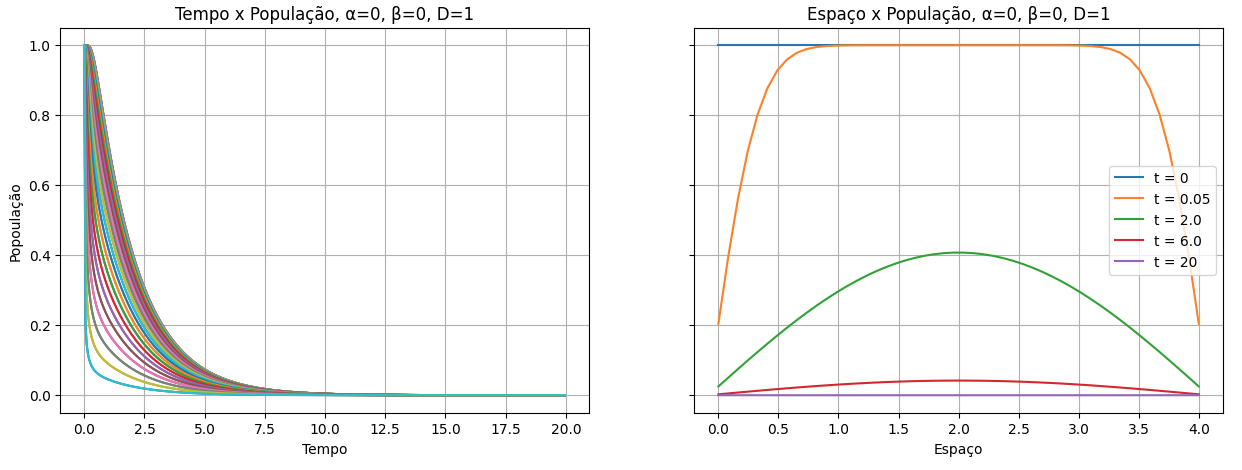
\includegraphics[scale=0.35]{L4-alpha0-beta0-D1}
	 	\caption{População na qual apenas o índice de difusão é atribuído, $D=1$, enquanto $\alpha = \beta = 0$. A população dentro da região vai a zero, toda ela escoando por difusão para fora da mancha. Aqui, $L=4$.}
	 	\label{fig:L4-alpha0-beta0-D1}
	 \end{figure}
 
 	\begin{figure}[h]
 		\centering
 		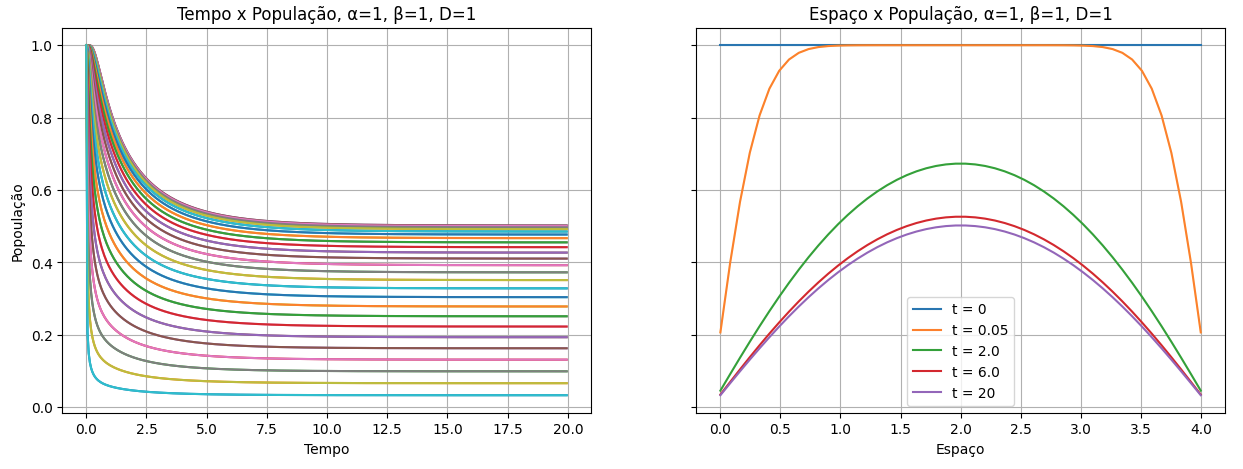
\includegraphics[scale=0.35]{L4-alpha1-beta1-D1}
 		\caption{População com índice de difusão atribuído, assim como os índices de competição e colaboração interna: $D=1$, $\alpha=1$, $\beta=1$. Aqui, $L=4$.}
 		\label{fig:L4-alpha1-beta1-D1}
 	\end{figure}
 	
 	\begin{figure}[h]
 		\centering
 		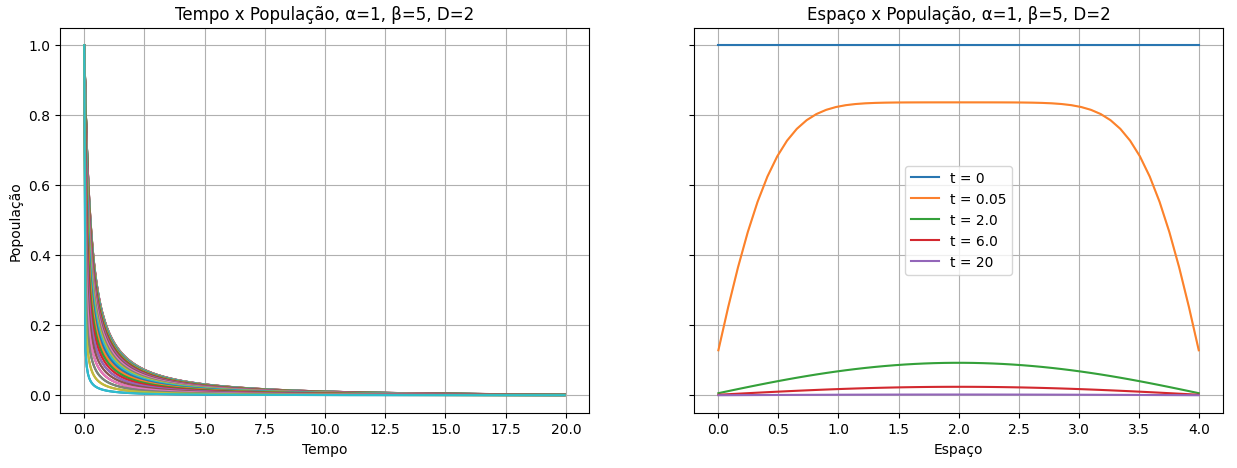
\includegraphics[scale=0.35]{L4-alpha1-beta5-D2}
 		\caption{População com índice de difusão atribuído, assim como os índices de competição e colaboração interna: $D=1$, $\alpha=1$, $\beta=5$. Índice de competição superior ao índice de colaboração, com resultados na redução da população sustentada pela mancha populacional. Aqui, $L=4$.}
 		\label{fig:L4-alpha1-beta5-D2}
 	\end{figure}
 
 	\begin{figure}[h]
 		\centering
 		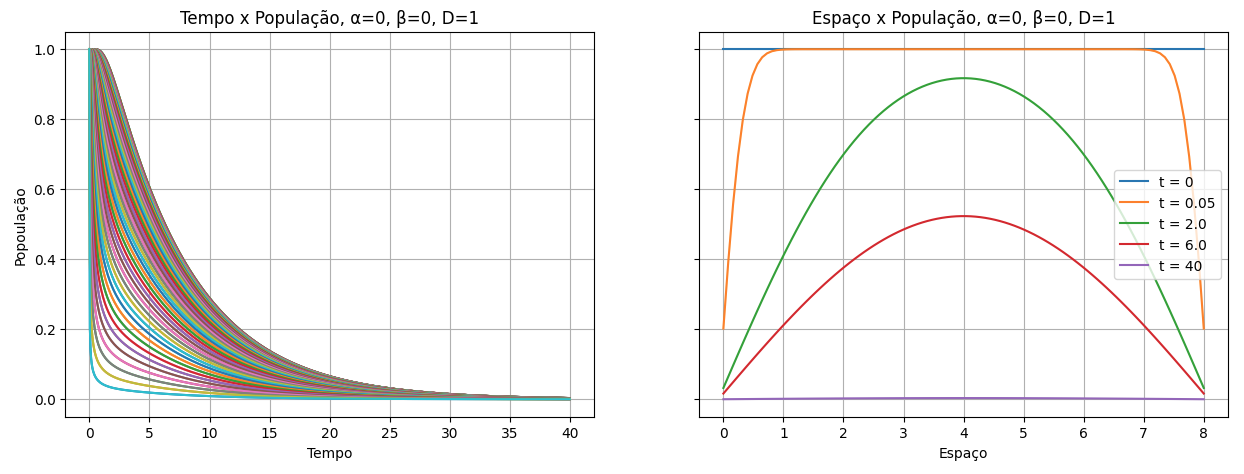
\includegraphics[scale=0.35]{L8-alpha0-beta0-D1}
 		\caption{Apenas com o índice de difusão atribuído, mesmo aumentando a área para $L=8$, e atribuindo $\alpha = \beta = 0$, $D = 1$, a população escoa e desaparece do mesmo jeito, apenas demora mais tempo para chegar a zero.}
 		\label{fig:L8-alpha0-beta0-D1}
 	\end{figure}
 
 	\begin{figure}[h]
 		\centering
 		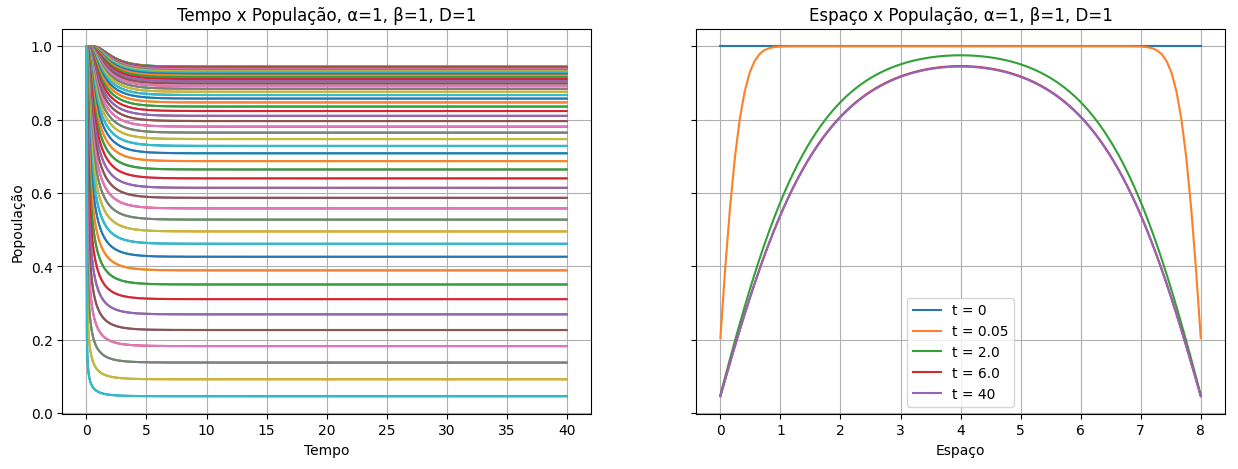
\includegraphics[scale=0.35]{L8-alpha1-beta1-D1}
 		\caption{População com índice de difusão atribuído, assim como os índices de competição e colaboração interna: $D=1$, $\alpha=1$, $\beta=1$. Aqui, $L=8$. Em uma área maior, fica claro que é possível sustentar uma população maior.}
 		\label{fig:L8-alpha1-beta1-D1}
 	\end{figure}
 
 	\begin{figure}[h]
 		\centering
 		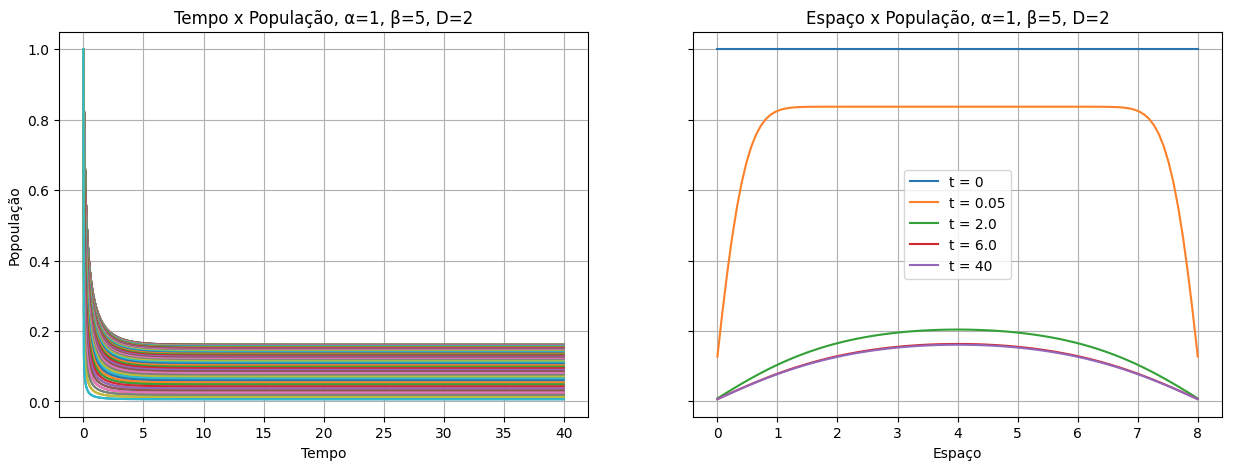
\includegraphics[scale=0.35]{L8-alpha1-beta5-D2}
 		\caption{População com índice de difusão atribuído, assim como os índices de competição e colaboração interna: $D=1$, $\alpha=1$, $\beta=5$. Aqui, $L=8$, permitindo sustentar uma população razoável, mesmo com alto índice de competição interna.}
 		\label{fig:L8-alpha1-beta5-D2}
 	\end{figure}
 
 	\begin{figure}[h]
 		\centering
 		\subfloat[\centering Apenas difusão]{{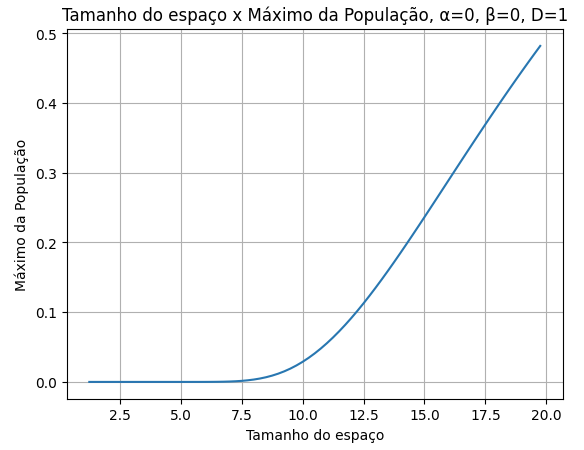
\includegraphics[scale=0.35]{Max-alpha0-beta0-D1}}}
 		\qquad
 		\subfloat[\centering Difusão, colaboração e competição]{{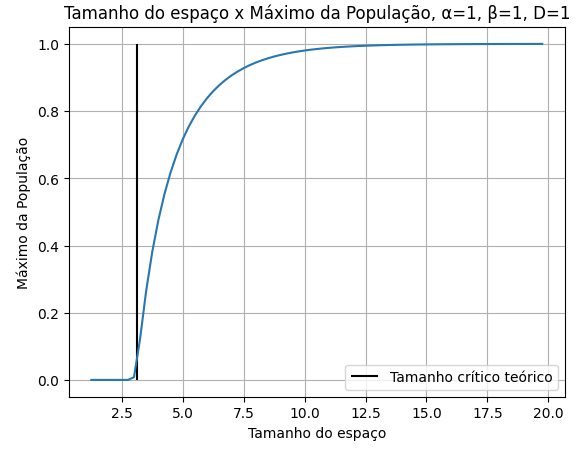
\includegraphics[scale=0.35]{TamanhoMax-alpha1-beta1-D1}}}
 		\caption{Avaliação da viabilidade de manutenção de população dependendo to tamanho do espaço da mancha. O caso (a), apenas difusão, não permite sustentar população alguma, independentemente do tamanho da área de mancha. Os tamanhos que apresentam alguma população, a partir de $L \geq 9$, significa apenas que, na simulação, não houve tempo suficiente para toda a população escoar. No caso (b), com competição e colaboração internas, a partir do espaço de suporte teórico, $L=\pi$, temos o aumento da população sustentável de forma consistente, até chegar ao máximo de $u = 1$, no longo prazo.}
 		\label{fig:Max-alpha0-beta0-D1}
 	\end{figure}
 
 	\begin{figure}[h]
 		\centering
 		\subfloat[\centering Ampliando fortemente fator de competição e ampliando fator de difusão.]{{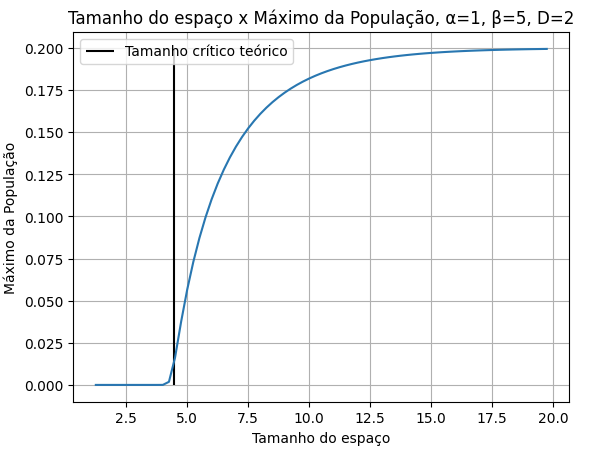
\includegraphics[scale=0.35]{TamanhoMax-alpha1-beta5-D2}}}
 		\qquad
 		\subfloat[\centering Ampliando fortemente o fator de competição e ainda mais fortemente o fator de difusão]{{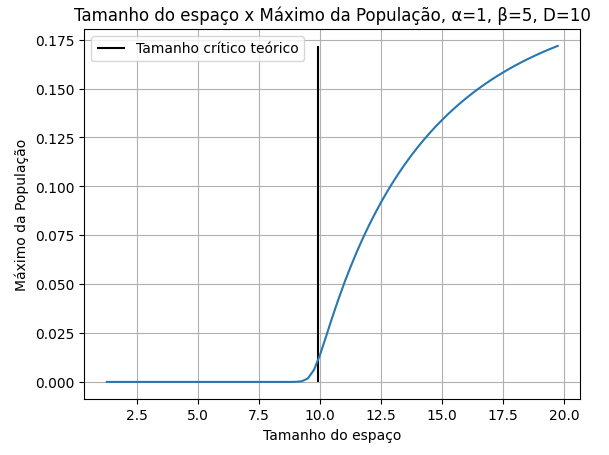
\includegraphics[scale=0.35]{TamanhoMax-alpha1-beta5-D10}}}
 		\caption{Quando ampliamos fortemente o fator de competição, para $\beta=5$, e o de difusão, para $D=2$, a partir do tamanho crítico teórico, uma população já começa a ser sustentável, mas cresce mais lentamente para uma população máxima, mas claramente inferior a 1. Quando ainda aumentamos mais o fator de difusão, $D=10$, a população ainda começa a ser sustentável a partir do limite crítico, e ainda cresce mais lentamente a partir daí, mas tende, claramente, para uma população máxima ainda mais reduzida.}
 		\label{fig:TamanhoMax-alpha1-beta5-D2}
 	\end{figure}
 
 	\begin{figure}[h]
 		\centering
 		\subfloat[\centering Grande índice de Competição]{{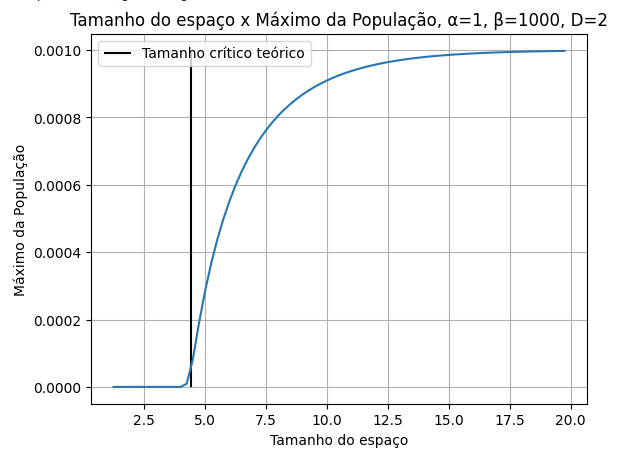
\includegraphics[scale=0.35]{TamanhoMax-alpha1-beta1000-D2}}}
 		\qquad
 		\subfloat[\centering Competição mais restrita, idêntica à colaboração]{{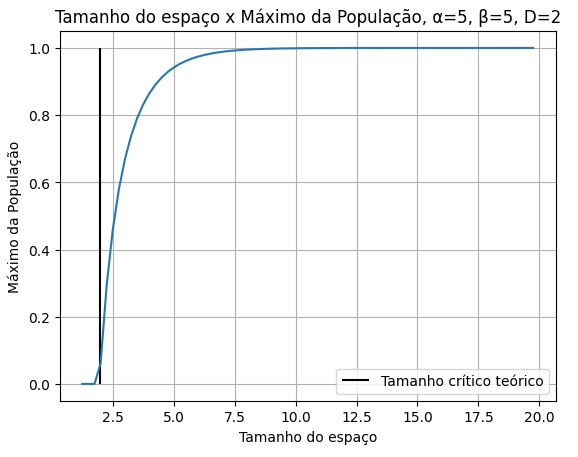
\includegraphics[scale=0.35]{TamanhoMax-alpha5-beta5-D2}}}
 		\caption{No caso (a), com a Difusividade controlada, $D=2$, Mas com uma grande competição interna, mil vezes superior à colaboração dentro da população, $\alpha=1$, $\beta=1000$, temos, ainda, uma população viável, mas ela é minúscula, seja de 1\% da inicial. No caso (b), temos um índice de competição maior, mas igual ao de colaboração, $\alpha = \beta = 5$, com a difusividade ainda controlada. Nesse caso, a população, após o Tamanho Crítico, aumentando esse espaço, chega ao máximo possível de $u = 1$, no longo prazo.}
 		\label{fig:TamanhoMax-alpha1-beta1000-D2}
 	\end{figure}

	\subsection{Análise de duas populações em competição}
	
	\paragraph{}
	Para a análise de duas populações, a EDP FKPP assume a forma vetorial. A equação vetorial, com duas populações de aves, segue, então, a as seguintes equações diferenciais:
	
	$$ \left[ \begin{array}{c}
		\frac{\partial u_1(x,t)}{\partial t} \\
		\frac{\partial u_2(x,t)}{\partial t} \end{array} \right]
	=
	\left[ \begin{array}{cc}
		u_1 \left[\alpha_1 - \beta_1 u_1  - \gamma_{12} u_2 \right] + D_1 \frac{\partial^2 u_1}{\partial x^2} \\
		u_2 \left[\alpha_2 - \beta_2 u_2  - \gamma_{21} u_1 \right] + D_2 \frac{\partial^2 u_2}{\partial x^2} \end{array} \right]$$
	
	\paragraph{}
	Como no método para uma única população, vamos usar o método das diferenças finitas para resolver essa EDP em um espaço limitado com condições de contorno de Dirichlet.
	
	$$u_i(x=0,L) = 0 $$
	
	\paragraph{}
	Para as diferenças finitas, podemos tomar:
	
	$$ \frac{\partial^2 u_i(x,t)}{\partial x^2} \approx \frac{u_i(x-dx,t) - 2u_i(x,t) + u_i(x+dx,t)}{dx^2}$$
	
	\paragraph{}
	Para resolver o sistema de Equações Diferenciais Parciais numericamente, podemos reduzi-la a um sistema de EDOs, com a aproximação para Laplaciano, conforme dado acima, e resolvendo em uma unica malha, em um eixo os valores de $u_i(x)$, representados como uma matriz em blocos $\left[\frac{\partial u_1(x,t)}{\partial t} \frac{\partial u_1(x,t)}{\partial t}\right]^T$ no lado esquerdo da igualdade que representa o sistema de EDOs.

	\paragraph{}	
	Para populações em competição, temos as seguintes condições:
	
	\begin{enumerate}
		\item $\gamma_1 \ne 0$
		\item $\gamma_2 \ne 0$
		\item $\alpha \ne 0$ e $\alpha \ne 1$
	\end{enumerate}

	\paragraph{}
	O que implica que em:
	
	$$\left[ \begin{array}{c}
		\frac{\partial u_1(x,t)}{\partial t} \\
		\frac{\partial u_2(x,t)}{\partial t} \end{array} \right]
	=
	\left[ \begin{array}{cc}
		u_1 \left[\alpha_1 - \beta_1 u_1  - \gamma_{12} u_2 \right] + D_1 \frac{\partial^2 u_1}{\partial x^2} \\
		u_2 \left[\alpha_2 - \beta_2 u_2  - \gamma_{21} u_1 \right] + D_2 \frac{\partial^2 u_2}{\partial x^2} \end{array} \right]$$
	
	\paragraph{}
	Temos:
	
	\begin{enumerate}
		\item $D_1 = 1$
		\item $D_2 = \kappa$
		\item $\alpha_1 = \beta_1 = 1$
		\item $\gamma_{12} = \gamma_1$
		\item $\alpha_2 = \beta_2 = \alpha$
		\item $\gamma_{21} = \alpha \gamma_2$
	\end{enumerate}
	
	\paragraph{}
	O que implica em:
	
	$$\left[ \begin{array}{c}
		\frac{\partial u_1(x,t)}{\partial t} \\
		\frac{\partial u_2(x,t)}{\partial t} \end{array} \right]
	=
	\left[ \begin{array}{cc}
		u_1 \left[1 - u_1  - \gamma_1 u_2 \right] +  \frac{\partial^2 u_1}{\partial x^2} \\
		u_2 \left[\alpha - \alpha u_2  - \alpha \gamma_2 u_1 \right] + \kappa \frac{\partial^2 u_2}{\partial x^2} \end{array} \right]$$
	
	\paragraph{}
	Que, por sua vez, implica em:
	
	$$\left[ \begin{array}{c}
		\frac{\partial u_1(x,t)}{\partial t} \\
		\frac{\partial u_2(x,t)}{\partial t} \end{array} \right]
	=
	\left[ \begin{array}{cc}
		u_1 \left[1 - u_1  - \gamma_1 u_2 \right] +  \frac{\partial^2 u_1}{\partial x^2} \\
		\alpha u_2 \left[1 - u_2  - \gamma_2 u_1 \right] + \kappa \frac{\partial^2 u_2}{\partial x^2} \end{array} \right]$$
	
	\paragraph{}
	Que é a versão adimensionalizada do problema, com o $\gamma_1$ e $\gamma_2$ devidamente isolados, de forma a analisar a competição entre as populações.
	
	\paragraph{}
	Existem algumas condições importante de $\gamma_1$, $\gamma_2$ e $L$ que vamos avaliar:
	
	\begin{itemize}
		\item Se $L$ for muito pequeno, ambas populações desaparecem.
		\item Se $L$ for grande o suficiente, $\gamma_1 < 1$ e $\gamma_2 < 1$, populações coexistem.
		\item Se  $L$ for grande o suficiente, $\gamma_1 < 1$ e $\gamma_2 > 1$, eliminação da espécie 2.
		\item Se   $L$ for grande o suficiente, $\gamma_1 > 1$ e $\gamma_2 > 1$, eliminação de qualquer das populações, dadas condições iniciais específicas.	
	\end{itemize}

	\paragraph{}
	Se a região for limitada, é testada aqui a condição na qual a primeira população é dominante, com $\gamma_1 < 1$ e $\gamma_2 > 1$, $\kappa = \alpha = 1$. Em todos os casos apresentados, os valores de $\alpha$ e $\kappa$ não são alterados, exceto se explicitamente declarados. Apenas variam-se os valores dos $\gamma_1$ e $\gamma_2$.
	
	\paragraph{}
	Todos os resultados das simulações podem ser vistas nas Figuras \ref{fig:Two-P-00-Diffusion-Time}, \ref{fig:Two-P-02-Diffusion-Space}, \ref{fig:Two-P-04-Competition-Time}, \ref{fig:Two-P-06-Competition-Space}, \ref{fig:Two-P-08-Coexistence-Time}, \ref{fig:Two-P-10-Coexistence-Space}, \ref{fig:Two-P-12-Elimination-Diffusion-Time}, \ref{fig:Two-P-14-Elimination-Diffusion-Space}, \ref{fig:Two-P-16-Elimination-Area-Time}, \ref{fig:Two-P-18-Elimination-Area-Space}, \ref{fig:Two-P-20-Population-Competition-Area-Time-Both} e \ref{fig:Two-P-21-Population-Competition-Time}. Os códigos fontes e os parâmetros para se chegar nesses resultados estão no Python Notebook \textit{Projeto-Modelagem Reação e Difusão - Duas populações.ipynb} em anexo.
	
	\begin{figure}[h]
		\centering
		\subfloat[\centering label 1]{{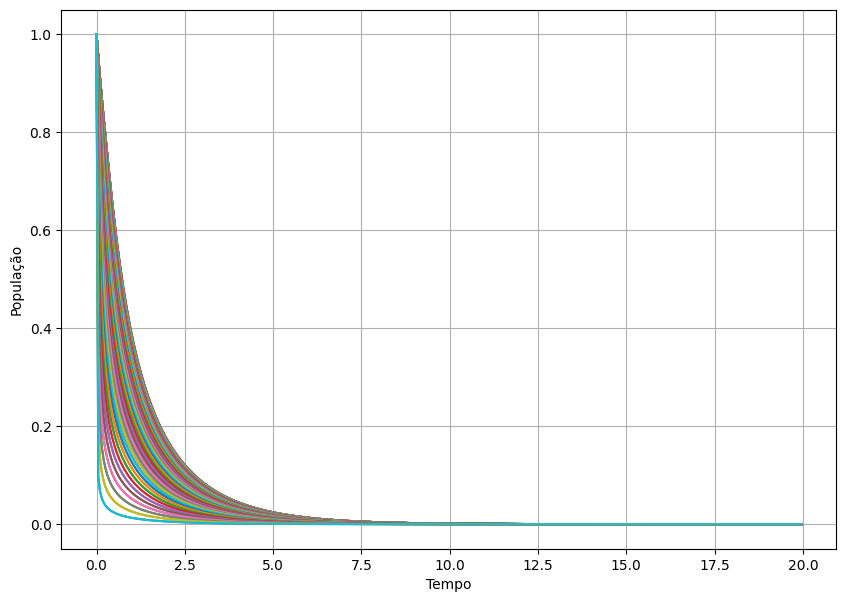
\includegraphics[scale=0.35]{Two-P-00-Diffusion-Time-1}}}
		\qquad
		\subfloat[\centering label 2]{{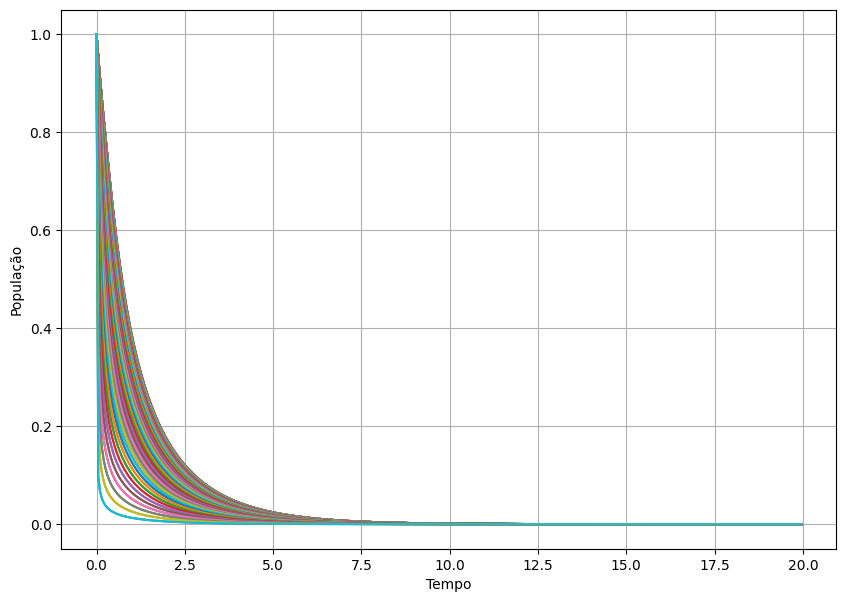
\includegraphics[scale=0.35]{Two-P-01-Diffusion-Time-2}}}
		\caption{Primeiro caso de duas populações. $L=4$, e é atribuído, apenas, os índices de difusão das duas populações, $D_1 = D_2 = 1$, $\gamma_1 = \gamma_2 = 0$. As duas populações não interagem entre si e ambas escoam até chegar a zero, na mancha florestada. Não é colocada leganda da posição das populações no gráfico, mas as populações mais baixas estão mais próximas dos cantos da mancha, enquanto as populações mais altas estão mais próximas ao centro. Esse padrão se repete em todos os gráficos temporais dos casos de duas populações.}
		\label{fig:Two-P-00-Diffusion-Time}
	\end{figure}	

	\begin{figure}[h]
		\centering
		\subfloat[\centering label 1]{{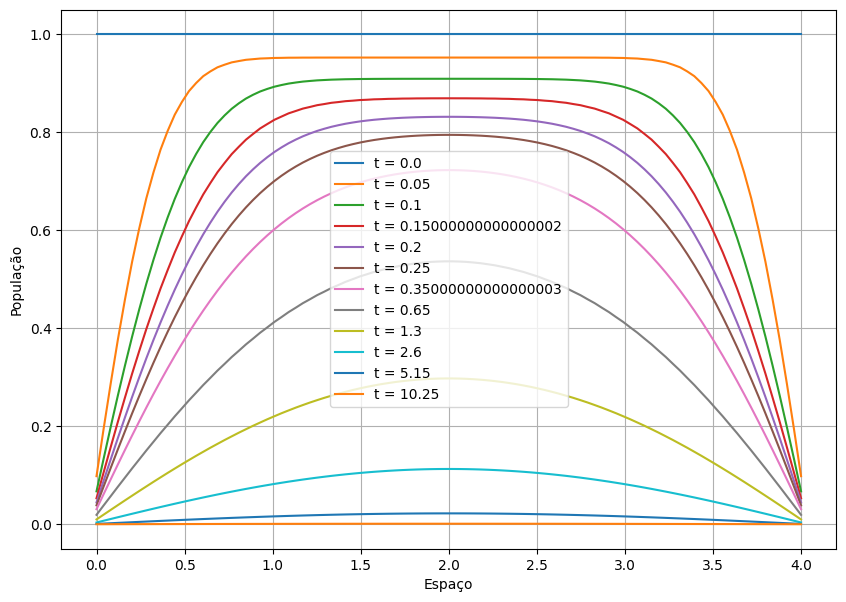
\includegraphics[scale=0.35]{Two-P-02-Diffusion-Space-1}}}
		\qquad
		\subfloat[\centering label 2]{{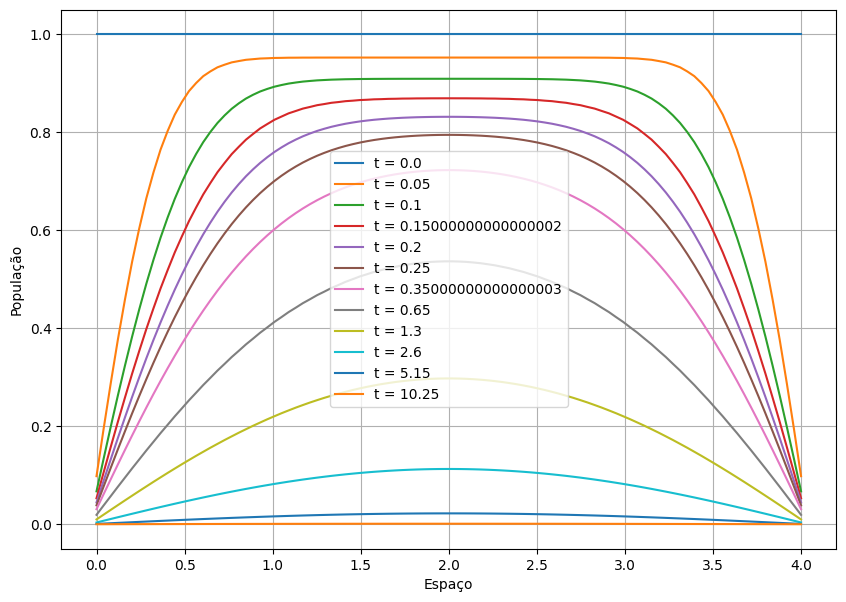
\includegraphics[scale=0.35]{Two-P-03-Diffusion-Space-2}}}
		\caption{Gráfico espacial para o primeiro caso de duas populações. $L=4$, $D_1 = D_2 = 1$, $\gamma_1 = \gamma_2 = 0$. Apesar de haver uma manutenção maior da população no centro, em toda a região, no longo prazo, ela vai a zero.}
		\label{fig:Two-P-02-Diffusion-Space}
	\end{figure}	
	
	\begin{figure}[h]
		\centering
		\subfloat[\centering Primeira População]{{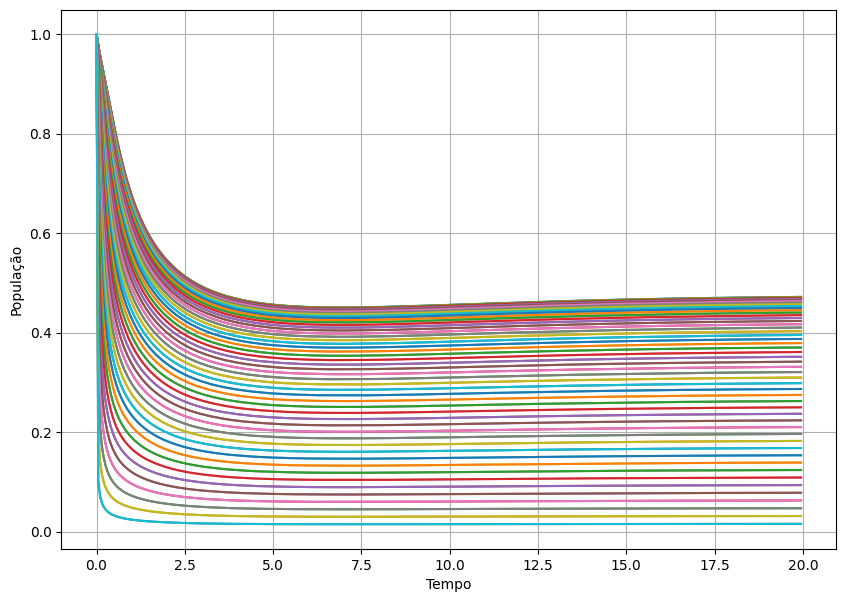
\includegraphics[scale=0.35]{Two-P-04-Competition-Time-1}}}
		\qquad
		\subfloat[\centering Segunda População]{{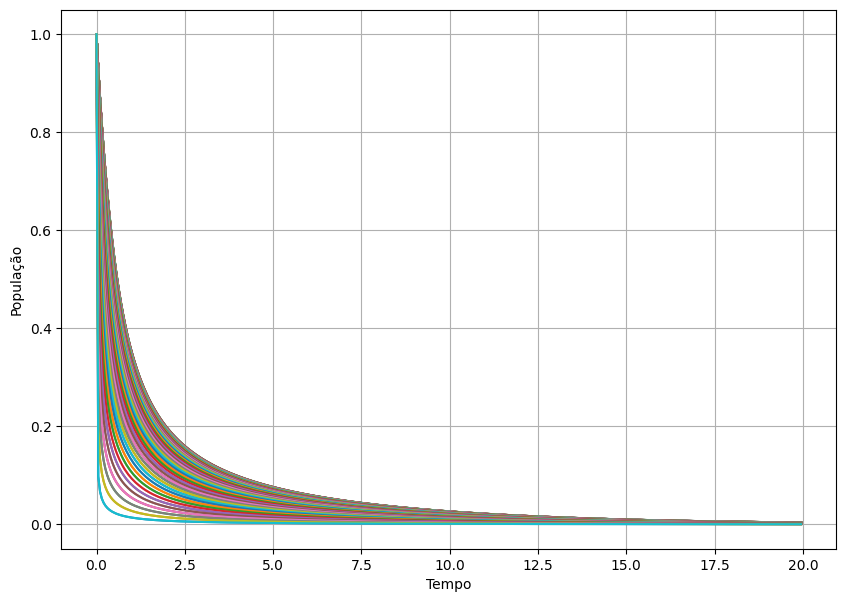
\includegraphics[scale=0.35]{Two-P-05-Competition-Time-2}}}
		\caption{Primeiro caso de competição, com eliminação da primeira população. Nesse caso, $L = 4$, $D_1 = D_2 = 1$,  $\gamma_1 = 0.5$, $\gamma_2 = 1.5$. A segunda população é fortemente afetada pela primeira - e é eliminada.}
		\label{fig:Two-P-04-Competition-Time}
	\end{figure}	
	
	\begin{figure}[h]
		\centering
		\subfloat[\centering Primeira População]{{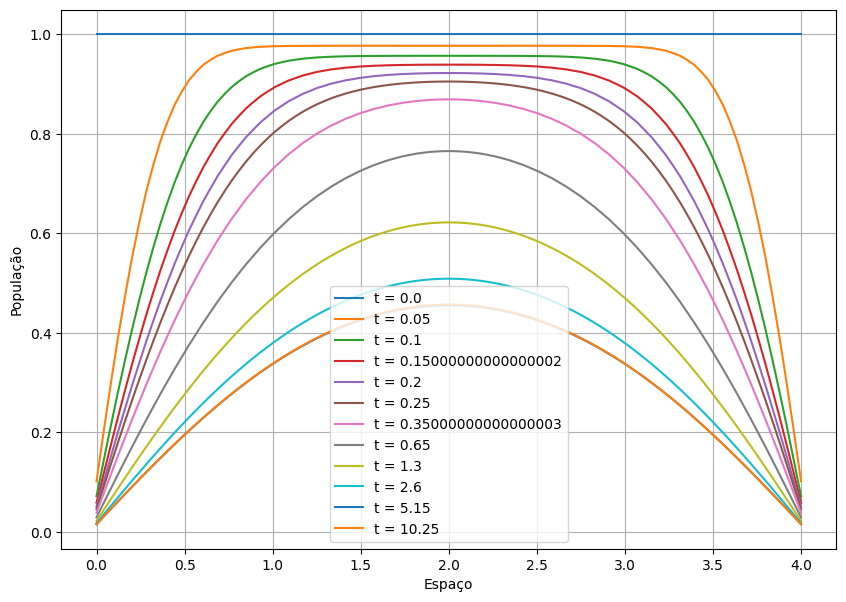
\includegraphics[scale=0.35]{Two-P-06-Competition-Space-1}}}
		\qquad
		\subfloat[\centering Segunda População]{{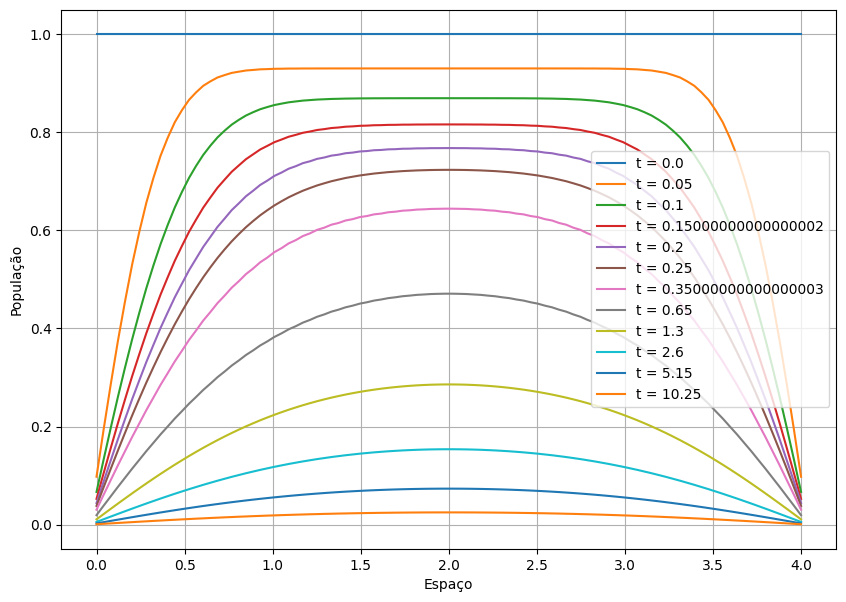
\includegraphics[scale=0.35]{Two-P-07-Competition-Space-2}}}
		\caption{Diagrama espacial do caso da Figura \ref{fig:Two-P-04-Competition-Time}.}
		\label{fig:Two-P-06-Competition-Space}
	\end{figure}	
	
	\begin{figure}[h]
		\centering
		\subfloat[\centering Primeira População]{{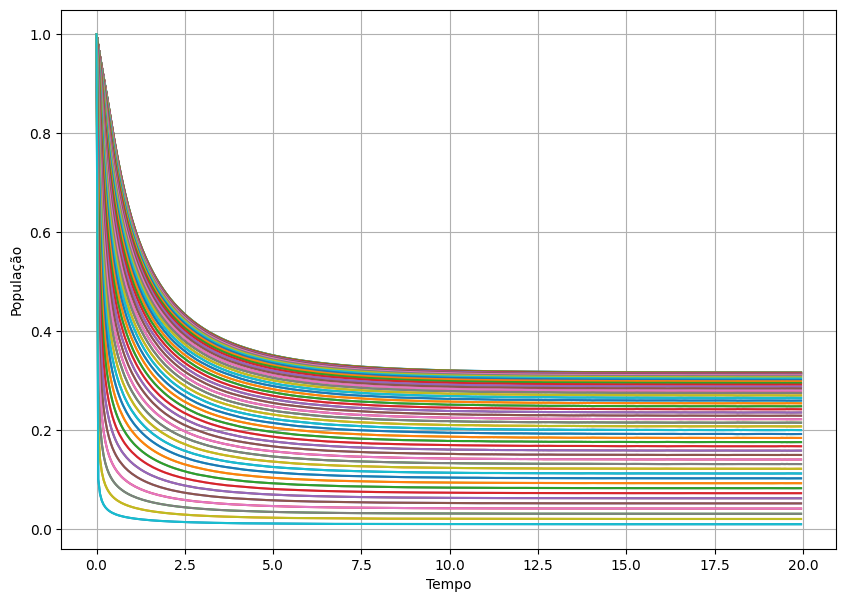
\includegraphics[scale=0.35]{Two-P-08-Coexistence-Time-1}}}
		\qquad
		\subfloat[\centering Segunda População]{{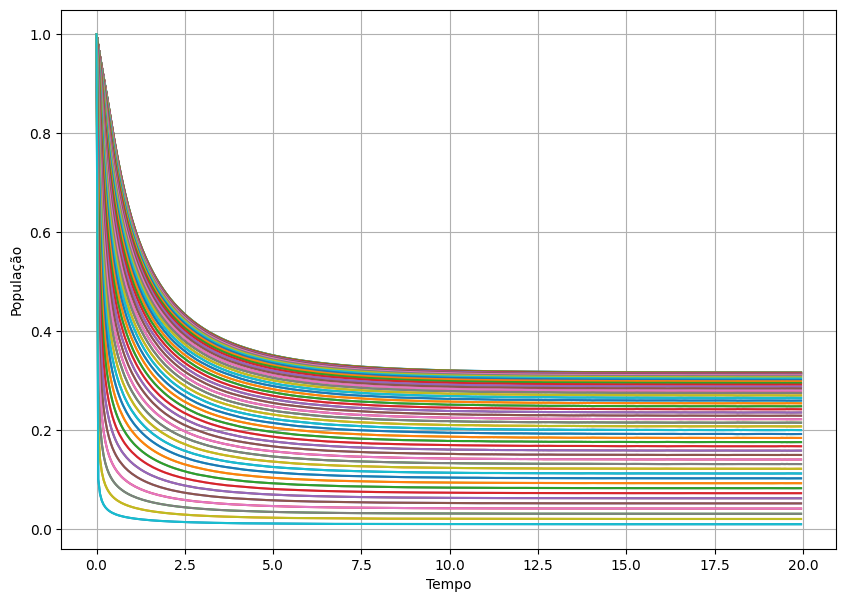
\includegraphics[scale=0.35]{Two-P-09-Coexistence-Time-2}}}
		\caption{Primeiro caso de coexistência entre as populações. Como $\gamma_1 = \gamma_2 = 0.5$, não há colaboração entre as populações, mas elas são relativamente insensíveis uma à outra no tocante à competição. Com $L = 4$, já é possível uma coexistència.}
		\label{fig:Two-P-08-Coexistence-Time}
	\end{figure}	
	
	\begin{figure}[h]
		\centering
		\subfloat[\centering Primeira População]{{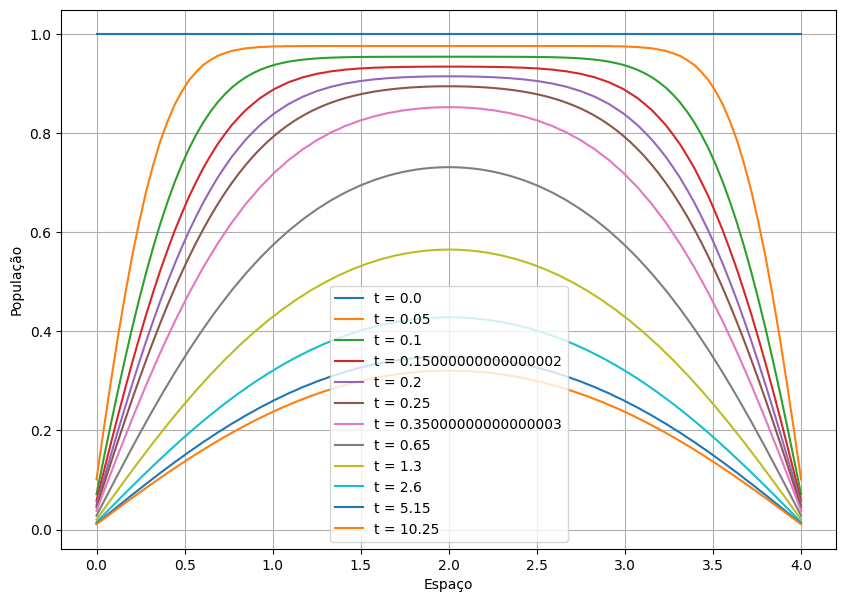
\includegraphics[scale=0.35]{Two-P-10-Coexistence-Space-1}}}
		\qquad
		\subfloat[\centering Segunda População]{{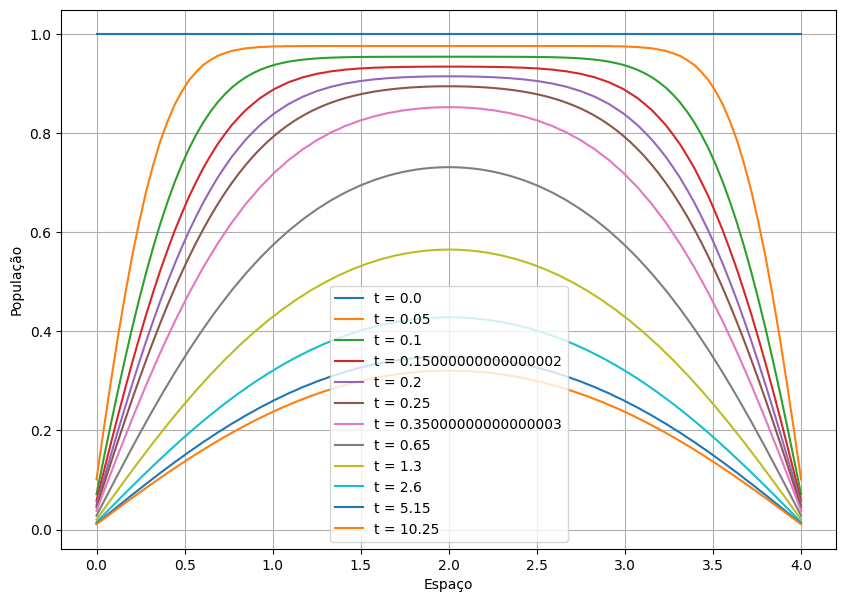
\includegraphics[scale=0.35]{Two-P-11-Coexistence-Space-2}}}
		\caption{Diagrama espacial do caso da Figura \ref{fig:Two-P-08-Coexistence-Time}}
		\label{fig:Two-P-10-Coexistence-Space}
	\end{figure}	
	
	\begin{figure}[h]
		\centering
		\subfloat[\centering Primeira População]{{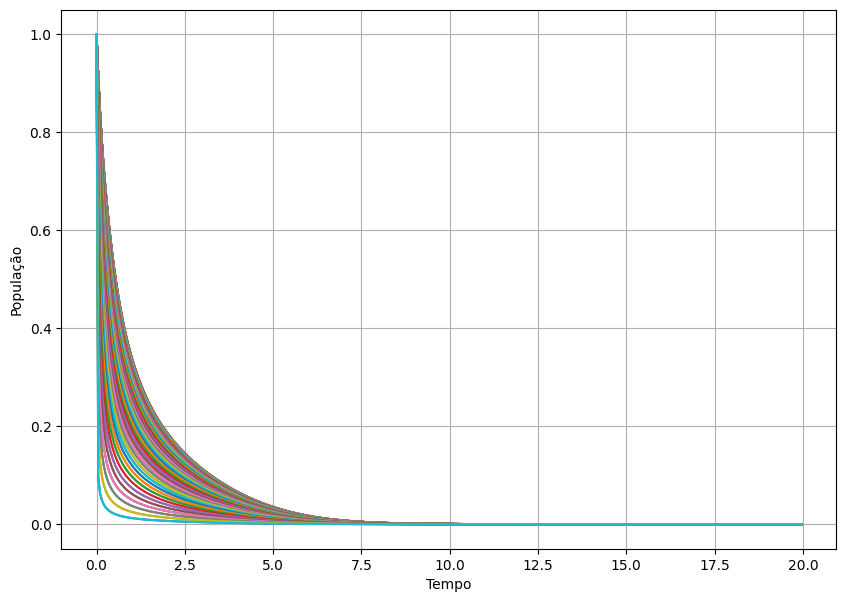
\includegraphics[scale=0.35]{Two-P-12-Elimination-Diffusion-Time-1}}}
		\qquad
		\subfloat[\centering Segunda População]{{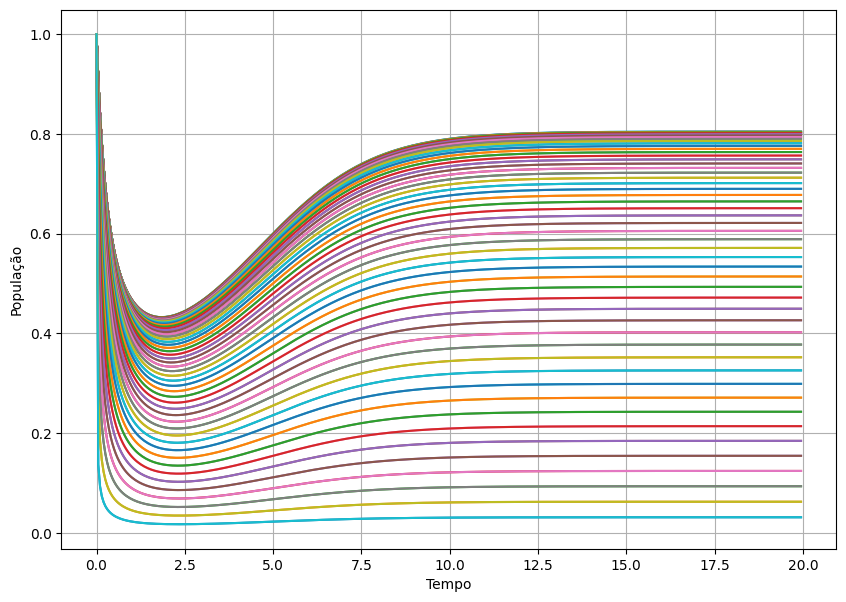
\includegraphics[scale=0.35]{Two-P-13-Elimination-Diffusion-Time-2}}}
		\caption{Caso especial, no qual os valores de $\gamma_1 = \gamma_2 = 2$, mas $\kappa = 0.5$, indicando que a População 2 tem menos interesse em sair da região da mancha, pois tem índice de difusividade igual à metade do índice de difusividade da População 1. $L=4$. Há um claro padrão de competição forte, no início da colonização, mas a População 1 é expulsa, e a População 2 se recupera e então se estabelece, no longo prazo, não restando membros da primeira população.}
		\label{fig:Two-P-12-Elimination-Diffusion-Time}
	\end{figure}	
	
	\begin{figure}[h]
		\centering
		\subfloat[\centering Primeira População]{{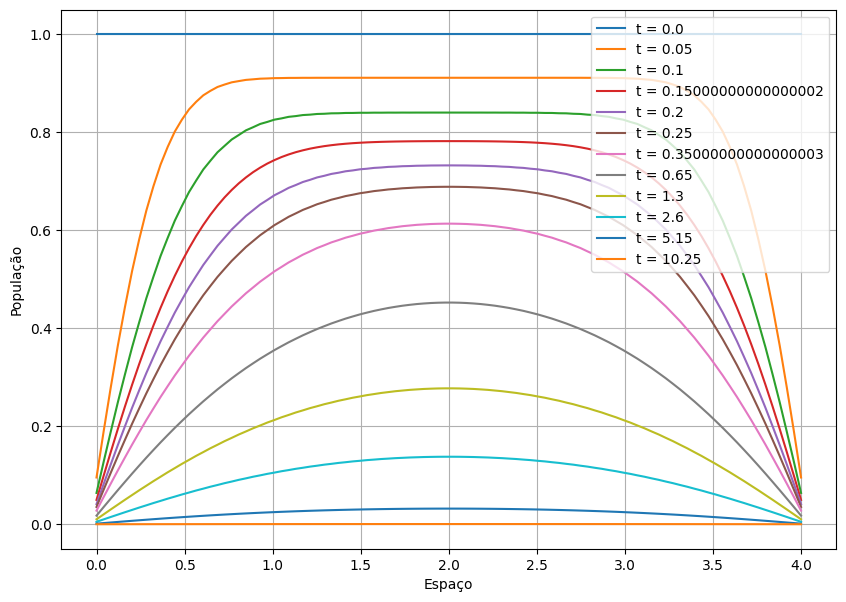
\includegraphics[scale=0.35]{Two-P-14-Elimination-Diffusion-Space-1}}}
		\qquad
		\subfloat[\centering Segunda População]{{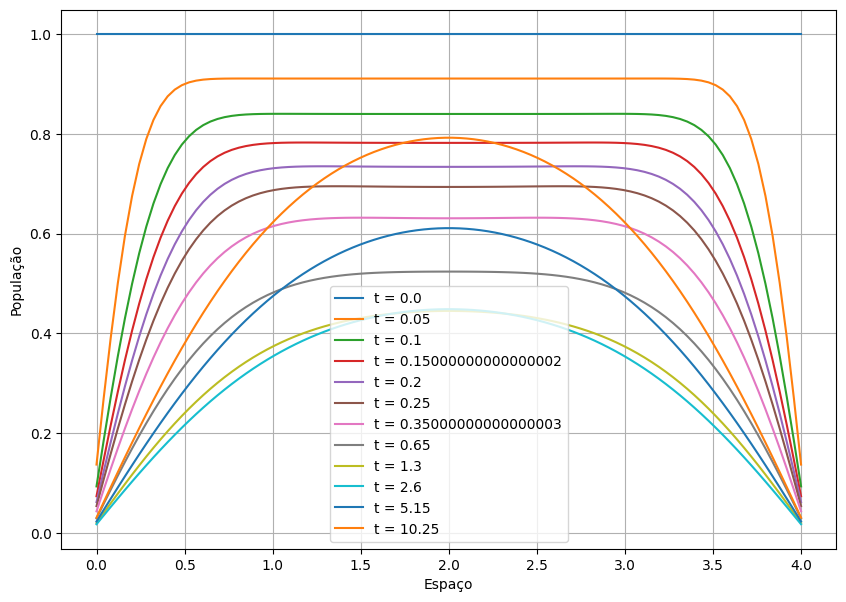
\includegraphics[scale=0.35]{Two-P-15-Elimination-Diffusion-Space-2}}}
		\caption{Gráfico espacial do caso da Figura \ref{fig:Two-P-12-Elimination-Diffusion-Time}. No caso (b), acima, é interessante ver que a População 2 chega a um mínimo, ainda mostrando efeitos da difusão, mas se recupera, com efeitos do crescimento da população e não fuga da região da mancha. Entretanto, a população nunca chega ao máximo inicial igual a 1.}
		\label{fig:Two-P-14-Elimination-Diffusion-Space}
	\end{figure}	
	
	\begin{figure}[h]
		\centering
		\subfloat[\centering Primeira População]{{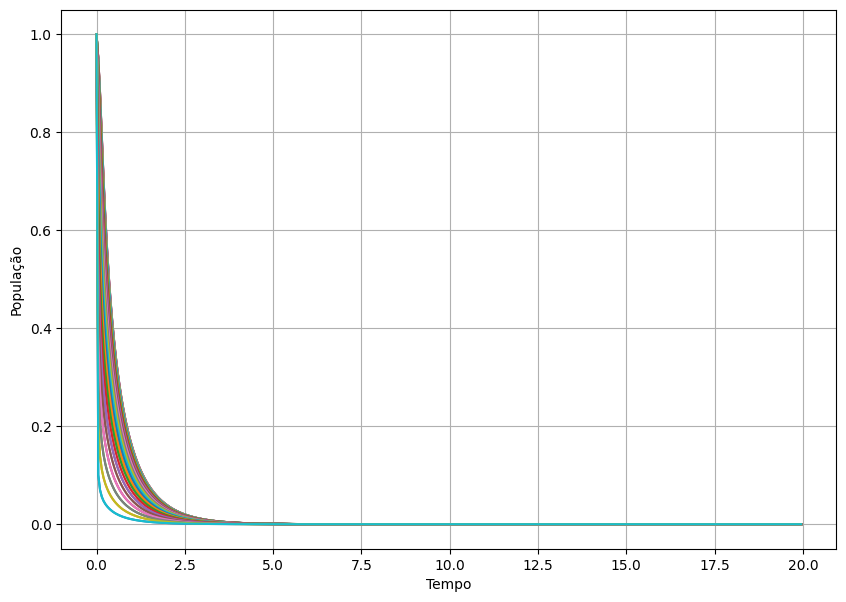
\includegraphics[scale=0.35]{Two-P-16-Elimination-Area-Time-1}}}
		\qquad
		\subfloat[\centering Segunda População]{{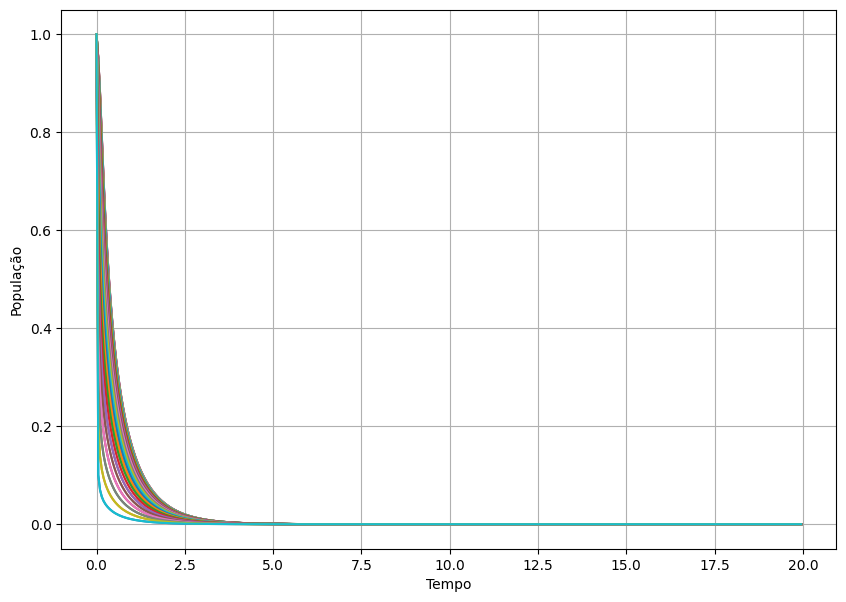
\includegraphics[scale=0.35]{Two-P-17-Elimination-Area-Time-2}}}
		\caption{Caso de duas populações abaixo do tamanho crítico teórico. Ambas populações são eliminadas. Aqui, $L = 2$, $\gamma_1 = \gamma_2 = 1$.}
		\label{fig:Two-P-16-Elimination-Area-Time}
	\end{figure}	
	
	\begin{figure}[h]
		\centering
		\subfloat[\centering Primeira População]{{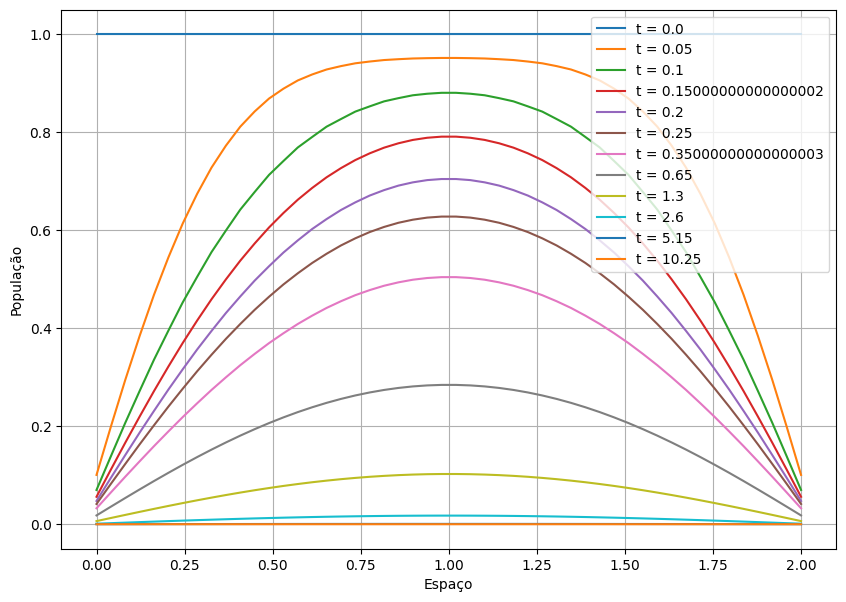
\includegraphics[scale=0.35]{Two-P-18-Elimination-Area-Space-1}}}
		\qquad
		\subfloat[\centering Segunda População]{{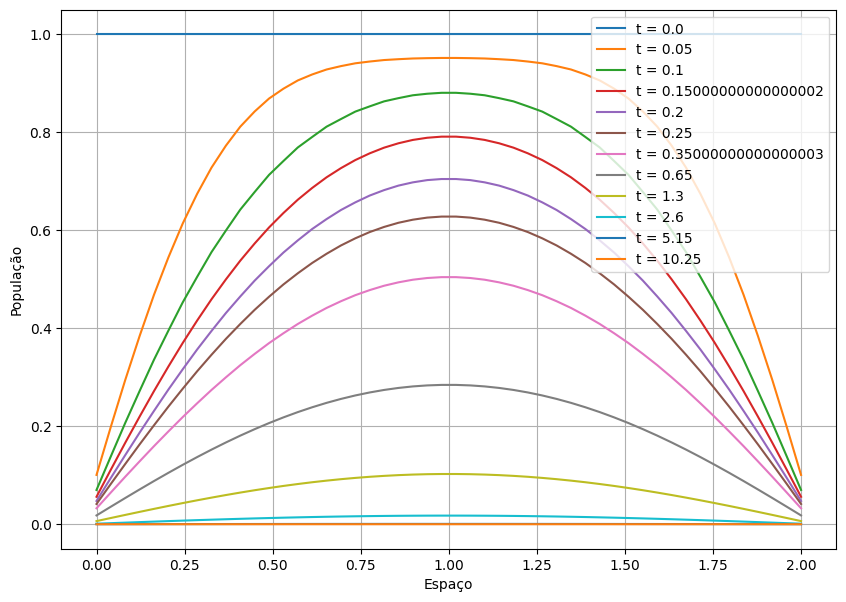
\includegraphics[scale=0.35]{Two-P-19-Elimination-Area-Space-2}}}
		\caption{Gráfico espacial para o caso apresentado na Figura \ref{fig:Two-P-16-Elimination-Area-Time}}
		\label{fig:Two-P-18-Elimination-Area-Space}
	\end{figure}	
	
	\begin{figure}[h]
		\centering
		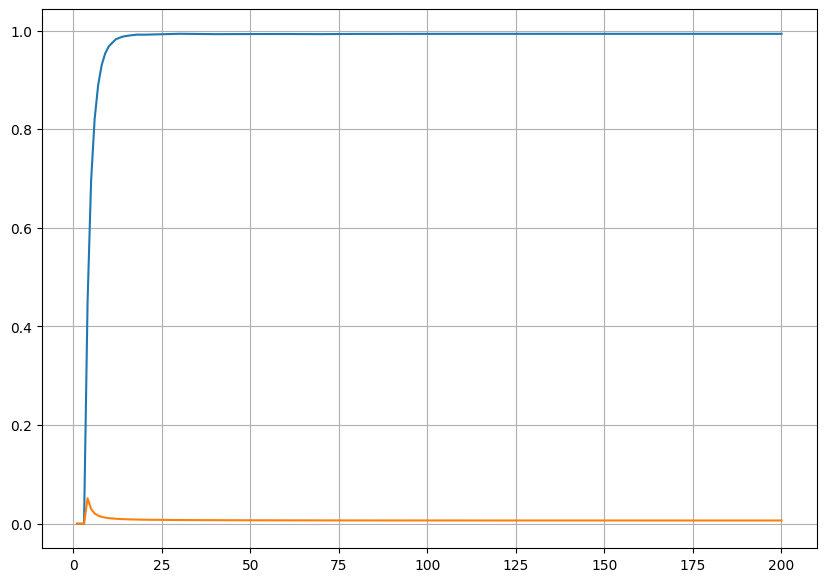
\includegraphics[scale=0.45]{Two-P-20-Population-Competition-Area-Time-Both}
		\caption{Caso de competição entre as duas populações - para diferentes $L$, que estão no eixo horizontal do gráfico. No eixo vertical temos a População 1, em azul, e População 2 em vermelho. Temos uma diferença mínima entre as tolerâncias de uma população com a outra. $\gamma_1 = 0.99$ e $\gamma_2 = 1.01$. Ainda assim, a População 1, no longo prazo, sempre domina, e apenas quando $L = 5$ temos uma coexistência razoável entre a População 1 e a População 2, sendo a População 1, nesse caso, nove vezes maior do que a População 2. A partir daí, a População 2 colapsa, se tornando marginal. Entretanto, na simulação, não é possível tomar um período $t$ infinito, então essa população marginal pode ser apenas o que sobra quando a simulação termina. Essa simulação possui o custo computacional bastante alto e, portanto, pode ser que haja erros sistemáticos por conta de a simulação ter sido feita em um período curto de tempo.}
		\label{fig:Two-P-20-Population-Competition-Area-Time-Both}
	\end{figure}	

	\begin{figure}[h]
		\centering
		\subfloat[\centering Primeira População]{{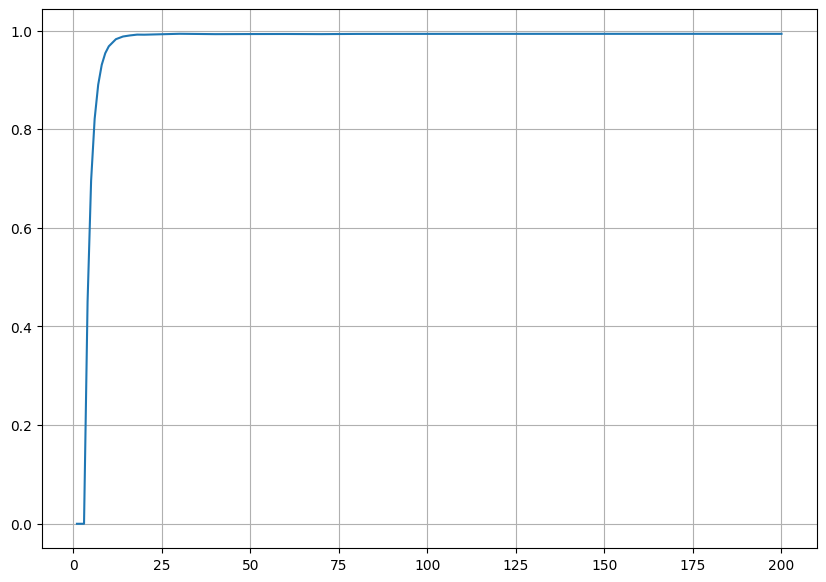
\includegraphics[scale=0.35]{Two-P-21-Population-Competition-Time-1}}}
		\qquad
		\subfloat[\centering Segunda População]{{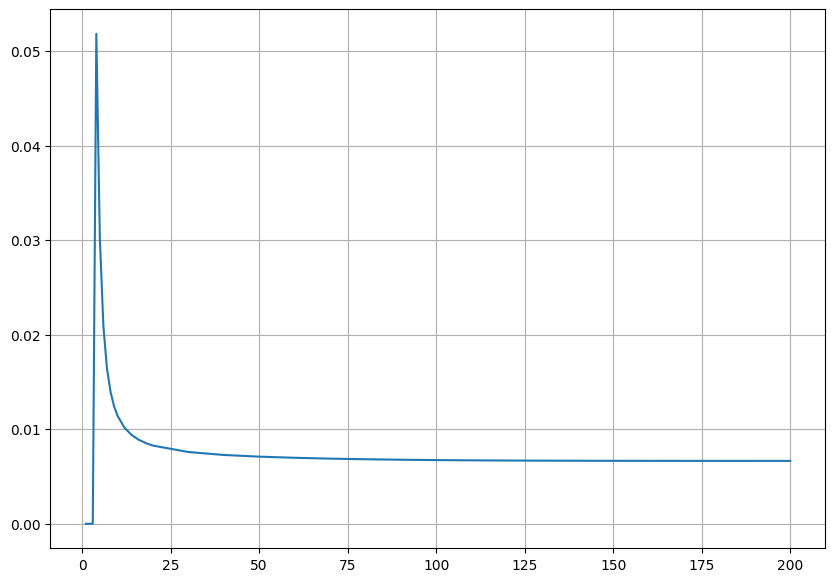
\includegraphics[scale=0.35]{Two-P-22-Population-Competition-Time-2}}}
		\caption{Gráficos das ~populações no longo prazo. A População 1 pouco percebe a competição com a População 2. A População 2 só tem relevância em manchas de tamanho pouco maior que o tamanho crítico. O custo computacional dessa simulação é alto, então é possível que após o pico da População 2, a queda de seu valor seja ainda mais pronunciado, se o tempo de simulação for mais longo para cada tamanho da manha L. No eixo horizontal de ambos os gráficos, temos o tamanho da mancha. No eixo vertical, temos a quantidade de população.}
		\label{fig:Two-P-21-Population-Competition-Time}
	\end{figure}	

	\section{Conclusões}
	
	\paragraph{}
	Foi possível avaliar o impacto do tamanho das manchas florestadas para a sustentação de populações dentro delas, considerando a reprodução, colaboração e competição interna das populações e a fuga dessas regiões, seguindo modelo de Reação e Difusão, da EDP FKPP. Para uma população, foi identificado com sucesso o tamanho crítico e a modelagem das características da população foi bem sucedida. 
	
	\paragraph{}
	Para duas populações os resultados não foram tão bem sucedidos. Dificuldades computacionais para identificar a área crítica e alta instabilidade dos parâmetros do sistema de EDPs tornou a análise difícil. Entretanto, foi perceptível que, dependendo da área da mancha florestada, populações em competição podem subsistir, uma em sombra da outra. Essa área, se for grande o suficiente para estar acima do tamanho crítico, permite uma coexistência mais bem sucedida da espécie desfavorecida, se tal área ainda for pequena o suficiente, para limitar o crescimento das duas populações e a sensitividade da segunda população em relação à primeira.
	
	\section{Referências Bibliográficas}
	
	\paragraph{Artiles W, Carvalho PG, Kraenkel RA. Patch-size and isolation effects in the Fisher-Kolmogorov equation.}
	J Math Biol. 2008 Oct;57(4):521-35. doi: 10.1007/s00285-008-0174-2. Epub 2008 May 9. PMID: 18465133.
\end{document}
